\documentclass{article}
\usepackage{eecstex}
\usepackage{pgfplots}

\renewcommand{\thesubsection}{\thesection.\arabic{subsection}}
\renewcommand{\thesubsubsection}{\thesubsection.\alph{subsubsection}}
\renewcommand{\labelenumi}{\arabic{enumi}.}
\newcommand{\F}{\mathcal{F}}
\newcommand{\sinc}{\operatorname{sinc}}
\newcommand{\rect}{\operatorname{rect}}


\title{EE 120 HW 09}
\author{Bryan Ngo}
\date{2021-03-28}

\begin{document}

\maketitle

\section{2D Filter}

\subsection{}

\begin{equation}
    h[n_1, n_2] = \frac{1}{5} (\delta[n_1, n_2] + \delta[n_1 - 1, n_2] + \delta[n_1 + 1, n_2] + \delta[n_1, n_2 - 1] + \delta[n_1, n_2 + 1])
\end{equation}

\subsection{}

Note that
\begin{align}
    h[n_1, n_2] &= \frac{1}{5} (\delta[n_1] \delta[n_2] + \delta[n_1 - 1] \delta[n_2] + \delta[n_1 + 1] \delta[n_2] + \delta[n_1] \delta[n_2 - 1] + \delta[n_1] \delta[n_2 + 1]) \\
    H(e^{j \omega_1}, e^{j \omega_2}) &= \frac{1}{5} (1 + e^{-j \omega_1} + e^{j \omega_1} + e^{-j \omega_2} + e^{j \omega_2}) = \frac{1}{5} (1 + 2\cos(\omega_1) + 2\cos(\omega_2)) \\
    |H(e^{j \omega_1}, e^{j \omega_2})| &= \frac{1}{5} (1 + 2|\cos(\omega_1)| + 2|\cos(\omega_2)|)
\end{align}
where we use the linearity and separation property of the 2D DTFT.

\begin{center}
    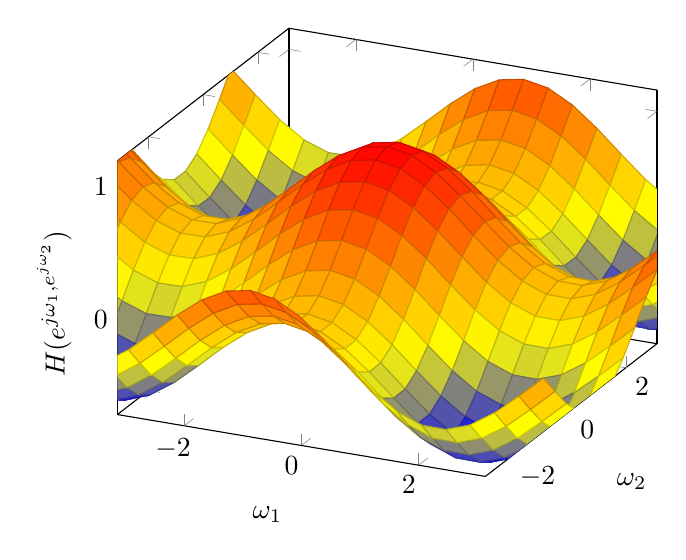
\begin{tikzpicture}
        \begin{axis}[
            xlabel=\(\omega_1\),
            ylabel={\(\omega_2\)},
            zlabel={\(H(e^{j \omega_1, e^{j \omega_2}})\)},
            xmin=-pi, xmax=pi,
            ymin=-pi, ymax=pi,
        ]
        \addplot3[
            surf,
        ]
        {(1 + 2 * cos(deg(x)) + 2 * cos(deg(y))) / 5};
        \end{axis}
    \end{tikzpicture}
    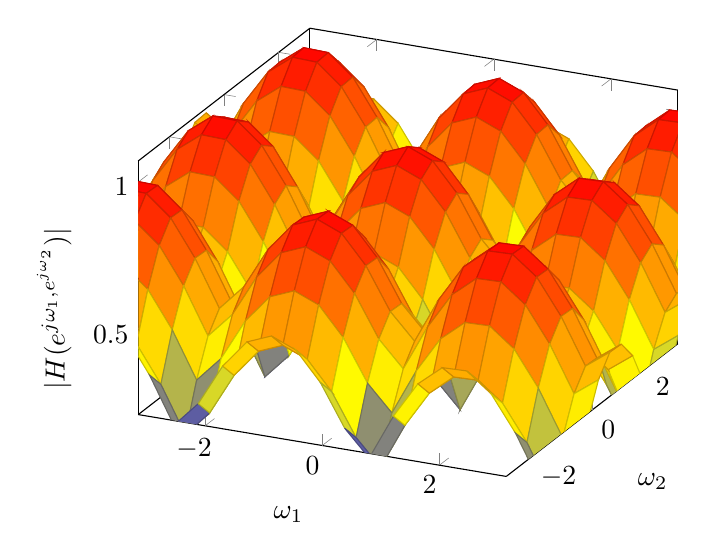
\begin{tikzpicture}
        \begin{axis}[
            xlabel=\(\omega_1\),
            ylabel={\(\omega_2\)},
            zlabel={\(|H(e^{j \omega_1, e^{j \omega_2}})|\)},
            xmin=-pi, xmax=pi,
            ymin=-pi, ymax=pi,
        ]
        \addplot3[
            surf,
        ]
        {(1 + 2 * abs(cos(deg(x))) + 2 * abs(cos(deg(y)))) / 5};
        \end{axis}
    \end{tikzpicture}
\end{center}

\section{FIR Filter}

\begin{equation}
    a[n] = \sum_{k \in [0, N]} a_k \delta[n - k]
\end{equation}

\subsection{}

By linearity of the CTFT,
\begin{equation}
    A(\omega) = \sum_{k \in [0, N]} a_k e^{-j \omega k}
\end{equation}
where the coefficients are the same as \(a[n]\).

\subsection{}

\subsubsection{}

\begin{align}
    c[n] &= (a \ast b)[n] \\
    &= \sum_{i \in [0, N]} a_i \delta[n - i] \ast \sum_{j \in [0, N]} b_j \delta[n - j] \\
    &= \sum_{i \in [0, N]} \sum_{j \in [0, M]} a_i b_j \delta[n - (i + j)]
\end{align}
Letting \(k = i + j\),
\begin{align}
    c[n] &= \sum_{i \in [0, N]} \sum_{k \in [i, M + i]} a_i b_{k - i} \delta[n - k] \\
    &= \sum_{k \in [0, M + i]} \sum_{i \in [0, N]} a_i b_{k - i} u[k - i] \delta[n - k] \\
    &= \sum_{k \in [0, M + N]} \underbrace{\sum_{i = \max\{0, k - M\}}^{\min\{k, N\}} a_i b_{k - i}}_{c_k} \delta[n - k]
\end{align}

\subsubsection{}

\begin{equation}
    C(e^{j \omega}) = A(e^{j \omega}) B(e^{j \omega}) = \sum_{k \in [0, M + N]} c_k e^{-j \omega k}
\end{equation}

\subsubsection{}

Since \(C\) is going to be a product of 2 polynomials, the result is going to be another polynomial in terms of \(e^{-j \omega}\), meaning its inverse CTFT will be in the form of an FIR filter with new coefficients.

\subsection{}

Evaluating a few different coefficients,
\begin{align}
    c_0 &= a_0 b_0 \\
    c_1 &= a_0 b_1 + b_1 a_0 \\
    &\vdots \\
    c_n &= a_0 b_n + a_1 b_{n - 1} + \cdots + a_n b_0 = \sum_{m \in [0, n]} a_m b_{n - m}
\end{align}

\section{Sampling Basics}

\begin{align}
    x_p(t) &= x(t) p(t) \\
    p(t) &= \sum_{k \in \Z} \delta(t - kT)
\end{align}

\subsection{}

We can use the cap to interlace the rectangles such that the left rectangle of the next duplicate touches the right edge of the triangle, or a shift of \SI{7}{\kilo\hertz}.
The minimum sampling rate is thus \SI{19}{\kilo\hertz}.

\subsection{}

\begin{center}
    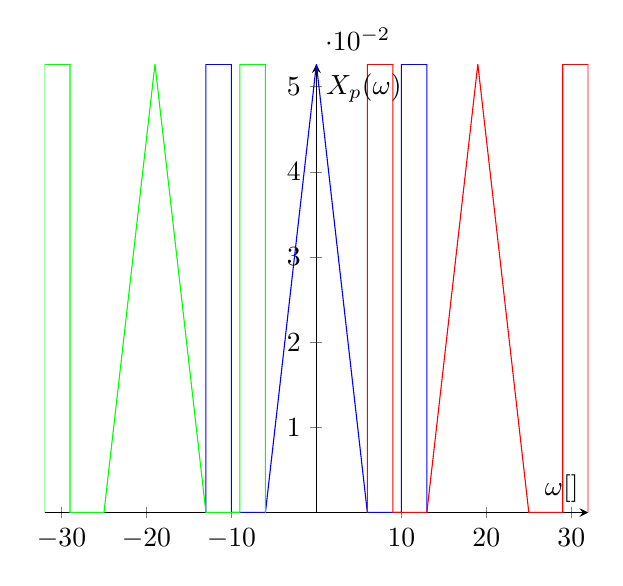
\begin{tikzpicture}
        \begin{axis}[
            xlabel={\(\omega [\si{\kilo\hertz}]\)},
            ylabel={\(X_p(\omega)\)},
            axis lines=middle,
            width=0.7\textwidth,
            height=\axisdefaultheight,
        ]
        \addplot[
            color=blue
        ]
        coordinates {
            (-13, 0) (-13, 1/19) (-10, 1/19) (-10, 0)
            (-6, 0) (0, 1/19) (6, 0)
            (10, 0) (10, 1/19) (13, 1/19) (13, 0)
        };
        \addplot[
            color=red
        ]
        coordinates {
            (6, 0) (6, 1/19) (9, 1/19) (9, 0)
            (13, 0) (19, 1/19) (25, 0)
            (29, 0) (29, 1/19) (32, 1/19) (32, 0)
        };
        \addplot[
            color=green
        ]
        coordinates {
            (-32, 0) (-32, 1/19) (-29, 1/19) (-29, 0)
            (-25, 0) (-19, 1/19) (-13, 0)
            (-9, 0) (-9, 1/19) (-6, 1/19) (-6, 0)
        };
        \end{axis}
    \end{tikzpicture}
\end{center}

\subsection{}

\begin{center}
    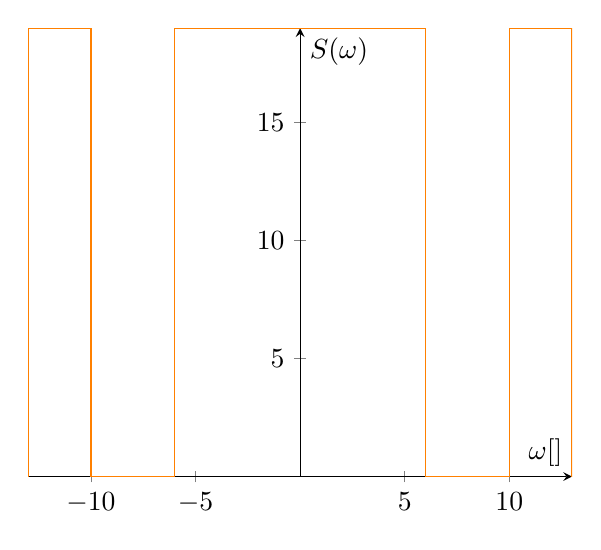
\begin{tikzpicture}
        \begin{axis}[
            xlabel={\(\omega [\si{\kilo\hertz}]\)},
            ylabel={\(S(\omega)\)},
            axis lines=middle,
            width=0.7\textwidth,
            height=\axisdefaultheight,
        ]
        \addplot[
            color=orange,
        ]
        coordinates {
            (-13, 0) (-13, 19) (-10, 19) (-10, 0)
            (-6, 0) (-6, 19) (6, 19) (6, 0)
            (10, 0) (10, 19) (13, 19) (13, 0)
        };
        \end{axis}
    \end{tikzpicture}
\end{center}

\end{document}
